\section{Implementing the DMP}
Having established the energy deposition in Eq.\ \eqref{R} and the
inequality in Eq.\ \eqref{DMP}, we now turn to translating
these terms into a functional form agreeable for use in a coding environment. 
Primarily, this involves approximating difficult functions such as the
exponential integrals $E_n(x)$ and $\mbox{Ei}(x)$, as well as numerically
evaluating
the various integrals over frequency.
Additionally, we desire a more general form of the DMP that can be
used in each cell to account for internal temperature gradients.

\subsection{Approximating $\tilde R$}
We address each of the terms of $\tilde R$ by breaking them up in Eq.
\eqref{DMPsplit}:
\begin{subequations}\label{DMPsplit}
\begin{align}
\tilde R(\Delta_x,\Delta_t)&\equiv\frac{f_0\Delta_t2\pi}{\Delta_x}
  \int_0^\infty\frac{\sigma_0B_u}{\hat\Sigma}\left(\frac{1}{2}-
    E_3(\hat\Sigma\Delta_x)\right)d\nu \label{DMP1}\\
  &+\frac{c_1f_0\Delta_t\sigma_p}{\lambda\Delta_x}(1-e^{-\lambda\Delta_x})
    \label{DMP2}\\
  &+\frac{f_0\Delta_t\sigma_p}{\lambda^2\Delta_x}\left[-\tilde A\Delta_x
    -L\frac{1}{\hat\Sigma}\left(\frac{1}{2}
    -E_3(\hat\Sigma\Delta_x)\right)\right] \label{DMP3}\\
  &\hspace{15pt}+\frac{f_0\Delta_t\sigma_pL}{\Delta_x\lambda^4}\hat\Sigma
    \bigg[e^{-\lambda\Delta_x}\mbox{Ei}[(\lambda-\hat\Sigma)\Delta_x] +
    e^{\lambda\Delta_x}\mbox{Ei}[-(\lambda+\hat\Sigma)\Delta_x] \label{DMP4} \\
  &\hspace{140pt} -2\mbox{Ei}(-\hat\Sigma\Delta_x)+ \nonumber
    \ln\frac{\hat\Sigma^2}{(\lambda+\hat\Sigma)|\lambda-\hat\Sigma|} \bigg].
\end{align}
\end{subequations}
While the terms in Eq. \eqref{DMPsplit} are generally listed in order of
increasing powers of $\lambda$ in the denominator, it should be noted that term
\eqref{DMP2} actually contains the term $\lambda^4$, because of the definition
of $c_1$ in Eq. (31) of \cite{WolLarDen}:
\[c_1=\frac{1}{1+2D\lambda}\frac{1}{\lambda^2}\left[A + 
  L\left(1+\frac{\hat\Sigma}{2\lambda}\ln\frac{|\lambda-\hat\Sigma|}{\lambda +
  \hat\Sigma} \right) \right],\hspace{10pt}\lambda\neq\hat\Sigma. \]

Inspection of the definition of $\lambda$ (repeated below) assists in assigning
the relative importance of terms in Eq. \eqref{DMPsplit}:
\[\lambda^2\equiv\frac{f_0\sigma_p + 1/c\Delta_t}{D}
  = \frac{f_0\sigma_p}{D} + \frac{1}{Dc\Delta_t} \]
  Since $f_0$ is restricted from zero to one, primary attention is turned to the
other terms in $\lambda^2$.


\subsubsection{Temperature}
Figure \ref{lambdaT} shows
$\lambda^2$ versus temperature for constants $\gamma=27$ keV$^3$/cm,
$c=3\times10^2$
cm/sh, and $\Delta_t=10^{-5}$ sh.  Additionally, it is assumed that the Planck
opacity
has the functional form
\begin{equation}
\sigma_p=\frac{15\gamma}{\pi^4T_0^3}\label{sigp assum},
\end{equation}
which may not be valid for many real materials, but serves as a
physically viable test case.

\begin{figure}[htb]
\centering
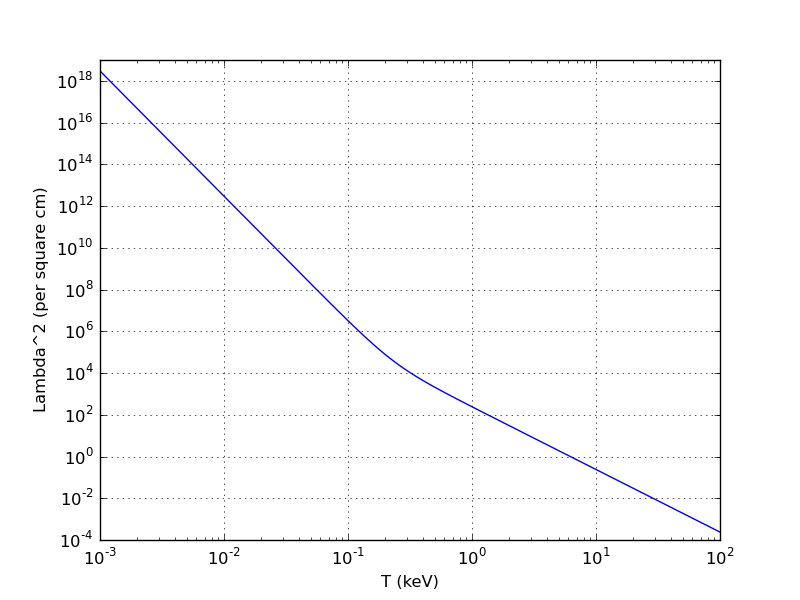
\includegraphics[width=0.7\linewidth]{lambdaT}
\caption{$\lambda$ as a function of material temperature}
\label{lambdaT}
\end{figure}
As can be seen, $\lambda^2$ falls as $T^6$ until an inflection point is reached
near $T=0.3$ keV, after which it falls as $T^3$.  It is worth noting that for
most of the range $0<T<1$ keV, $\lambda^2$ is very large.  As such, terms in
$\tilde R$ with exponential values of $\lambda^2$ will be vanishingly small for
most temperatures below 1 keV; however, further analysis needs to be done in
order to determine how many terms in $\tilde R$ can be neglected because of
their insignificance next to other terms because of temperature.


\subsubsection{Time Step}
It is also enlightening to consider the effect of an increasing time step on
$\lambda^2$.  Since a 1/$\Delta_t$ term is in the numerator of $\lambda^2$, a
term with 1/$\lambda^2$ varies as $O(\Delta_t)$ as $\Delta_t \to \infty$.  In
Eq.\
\eqref{DMPsplit}, a $\Delta_t$ term already exists in the numerator of each
term.
Thus, term\ \eqref{DMP1} varies linearly with $\Delta_t$.  The term with the
next lowest order of $\lambda$, term\ \eqref{DMP3}, has a 1/$\lambda^2$
coefficient, meaning it varies as $\Delta_t^2$.  Terms\ \eqref{DMP2} and\
\eqref{DMP4} vary as $\Delta_t^{5/2}$ and $\Delta_t^3$ respectively.  Thus, as
the time step becomes large, the latter terms in Eq.\ \eqref{DMPsplit} become
more significant.

It is unclear from the influence of both $T$ and $\Delta_t$ what terms in
$\tilde R$ are necessary to maintain accuracy for a variety of conditions. 
Future work will be done to evaluate these terms independently in the limit as
$\Delta_t\to 0, \infty$.  For the sake of the current work,
we turn to numerical methods to evaluate the relative impact of the terms,
acknowledging the results are specific to this particular sample problem.

\subsubsection{Numerical Comparison}
Given the difficulty in analytically determining the importance of the terms in
$\tilde R$, we performed a numerical study similar to that in \cite{WolLarDen},
using the
same values for $\sigma_p$, $\beta$, and $D$.  In each run, one of the terms
in
Eq.\ \eqref{DMPsplit} was set to zero, with the exception of the first term,
which si the dominant contributor to $\tilde R$ for this problem.  Instead, the
first term
was reduced by an order of magnitude in order to show how it scales the overall
calculation of the
discrete maximum principle.  The results are shown in Figures \ref{numR} through
\ref{numR_relErr} with the following definition for each case:
\begin{center}
\begin{tabular}{c c l}
Run & Modified Term & Modification  \\ \hline \medskip
All Terms & None &  None\\ \medskip
Case 0    & $\int_0^\infty2\pi B_u\frac{\sigma_0}{\hat\Sigma}
  \left(\frac{1}{2}-E_3(\hat\Sigma\Delta_x)\right)\ d\nu $& $\to 0$ \\ \medskip
Case 1    & $\frac{\sigma_p}{\lambda^2}L\frac{1}{\hat\Sigma}
  \left(\frac{1}{2}-E_3(\hat\Sigma\Delta_x)\right)\;$& \textdiv 10  \\ \medskip
Case 2    & $\frac{c_1\sigma_p}{\lambda\Delta_x} 
  \left(1-e^{-\lambda\Delta_x}\right) $ &$\to0$ \\ \medskip
Case 3    & $\frac{\sigma_p}{\lambda^2}A\Delta_x $ &$\to0$  \\ \medskip
Case 4    & Term\ \eqref{DMP4} & $\to0$  \\ \medskip
Case 5    & Cases 2, 3, and 4 combined &$\to0$
\end{tabular}
\end{center}
As can be seen, Case 1 had the greatest impact, followed by
Case 0, with Case 3 in a distant third place.  The terms
eliminated in Cases 2 and 4, on the other hand, seem to have very little real
impact on the overall location of the maximum principle violations.  In order to
minimize computation,
the terms left out in cases 2 and 4 will be left out of the
implementation of the DMP.

\begin{figure}[H]
\centering
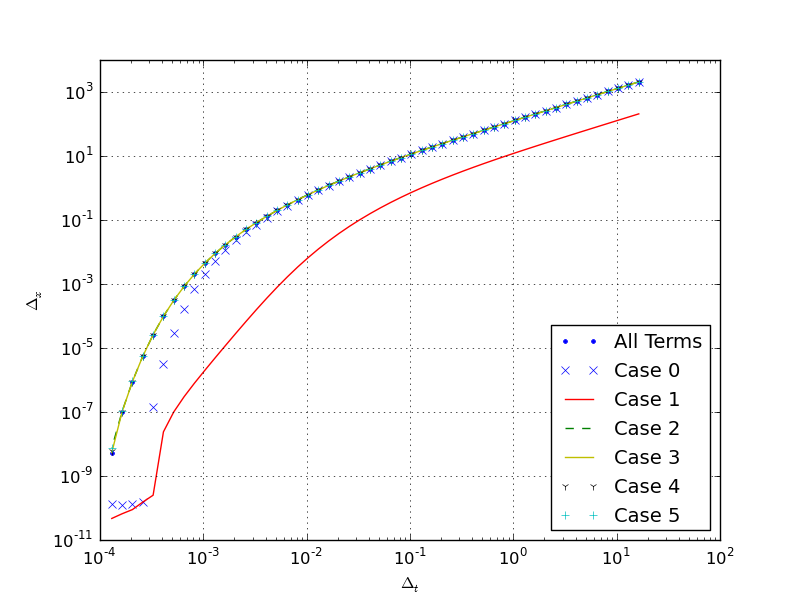
\includegraphics[width=0.7\linewidth]{numR}
\caption{Energy Deposited, $R$}
\label{numR}
\end{figure}

\begin{figure}[H]
\centering
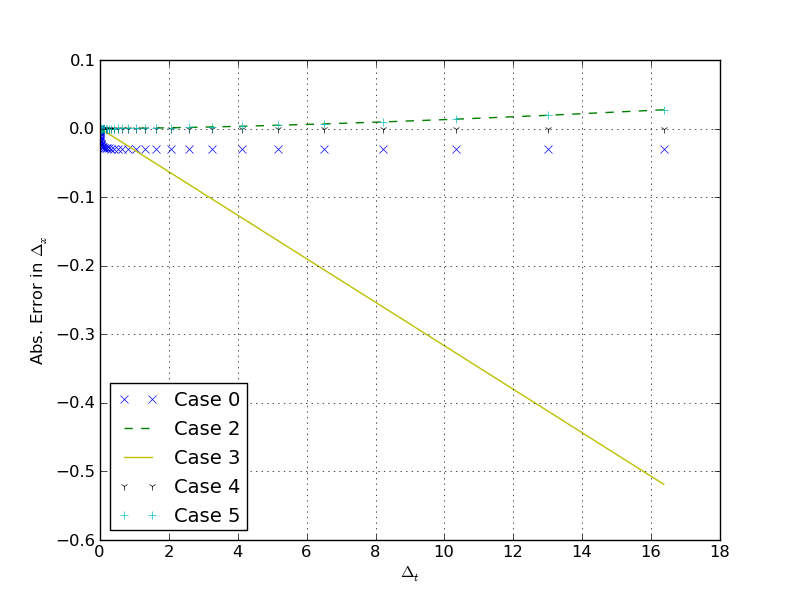
\includegraphics[width=0.7\linewidth]{numR_absErr}
\caption{Absolute Error in $R$ Approximations}
\label{numR_absErr}
\end{figure}

\begin{figure}[H]
\centering
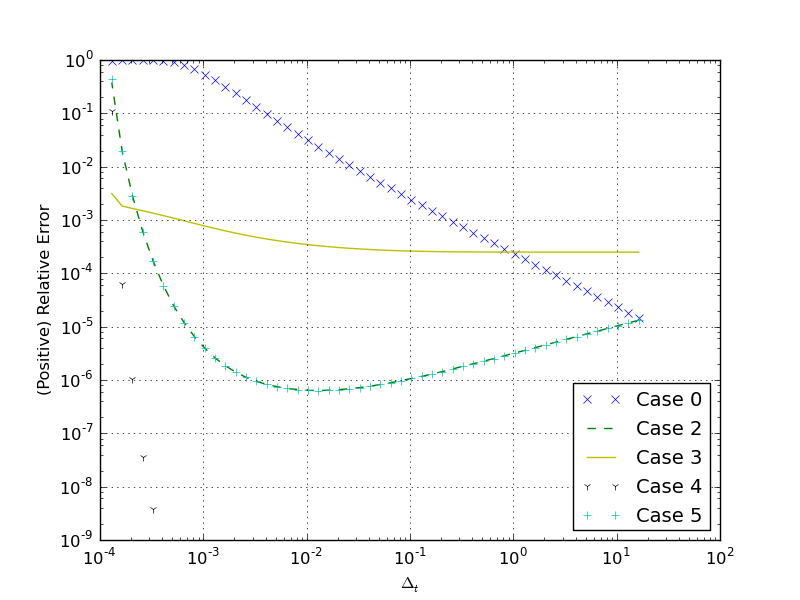
\includegraphics[width=0.7\linewidth]{numR_relErr}
\caption{Relative Error in $R$ Approximations}
\label{numR_relErr}
\end{figure}

\subsubsection{Frequency Discretization of $\tilde R$}
Removing the two least-significant terms as discussed above, $\tilde R$ is
approximated as
\begin{equation}
\tilde R\simeq\frac{f_0\Delta_t}{\Delta_x}\left(\zeta -
  \frac{\sigma_p}{\lambda^2}\tilde A\Delta_x - 
  \frac{\sigma_p}{\lambda^2}\frac{1-f_0}{-D}\zeta\right), \label{R approx}
\end{equation}
where we define the uncollided flux integral
\begin{equation}
\zeta\equiv\int_0^\infty 2\pi\sigma_0B_u\left[
  \frac{1}{2}-E_3(\hat\Sigma\Delta_x)\right]\ d\nu. \label{UncollidedFlux}
\end{equation}

Using the multigroup approximation described in Appendix \ref{apxMultigroup}
and the computational solution for $E_3(\hat\Sigma\Delta_x)$ discussed in
Appendix \ref{apxEn}, Eq.\ \eqref{R approx} becomes computationally
straightforward.

An interesting result occurs when the multigroup approximation is applied to
the estimate $\tilde R$.  In Figure \ref{CMP_DMP} we note that the analytic
Discrete Maximum
Principle curve, obtained from a numerical integral over frequency in
\texttt{Matlab}, diverges from the experimental data somewhere between
$\Delta_t$ of 0.001 and 0.01 shakes.  This suggests that the analytic discrete
maximum principle is not conservative enough to match experiment.  However,
when the multigroup approximation is applied, the curve matches much more
closely, as shown in Figure \ref{mg_DMP}.  It is not entirely surprising that
the multigroup approximation is more accurate, since
the experimental results were generated using a 100-group frequency grid in
\texttt{milagro}.
\begin{figure}[htb]
\centering
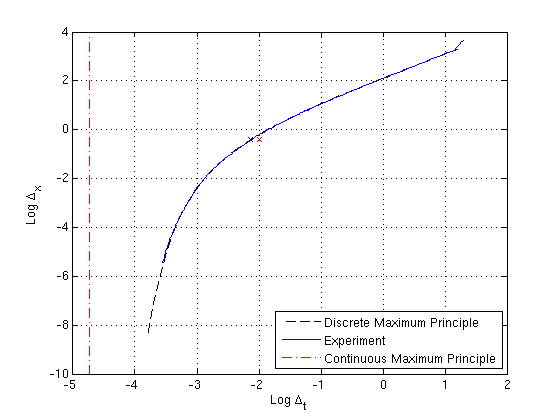
\includegraphics[width=0.7\linewidth]{grossMG}
\caption{Multigroup Approximation of DMP}
\label{mg_DMP}
\end{figure}


\subsubsection{Grey Case}
Because of the structure of the use codes that the DMP will likely be used in,
we deem it essential to construct an algorithm that will handle the 1-group gray
case as well as the multifrequency case.  A derivation of the discrete maximum 
principle for the frequency-independent gray case is derived here that takes
the same form as Eq.\ \eqref{DMP}.

We start with the gray transport equation in one dimension in \cite{FleckCumm},
which assumes that frequency is independent of angle and can be integrated out:
\begin{equation}
\frac{1}{c}\frac{\partial I}{\partial t} + \mu\frac{\partial I}{\partial x} +
  \sigma_0 I = \sigma_0(1-f_0)\frac{1}{2}\int_{-1}^1 I\ d\mu + \sigma_0f_0
  \frac{acT_0^4}{2},
  \label{1Dgreytransport}
\end{equation}
with the boundary and initial conditions
\begin{align}
I(0,\mu,t)&=\frac{ac}{2}T_u^4\equiv B_u,\hspace{20pt}0<\mu\leq1, 0\leq t,\\
I(X,\mu,t)&=\frac{ac}{2}T_0^4\equiv B_0,\hspace{20pt}-1<\mu\leq0, 0\leq t,\\
I(x,\mu,0)&=\frac{ac}{2}T_R^4\equiv B_R,\hspace{20pt}0\leq x\leq\infty, |\mu|<1.
  \label{1Dgreyinitcond}
\end{align}
Implicitly time differencing Eq.\ \eqref{1Dgreytransport}, we arrive at
\begin{equation}
\frac{1}{c}\frac{I_1-I_0}{\Delta_t}+\mu\frac{\partial I_1}{\partial x} + 
  \sigma_0 I_1 = \sigma_0(1-f_0)\frac{1}{2}\int_{-1}^1I_1\ d\mu + \sigma_0f_0
  \frac{acT_0^4}{2}
  ,\label{1Dgreytimediff}
\end{equation}
where $I_1\equiv I(t_1)$.  Using the initial condition in Eq.\ \eqref{1Dgreyinitcond},
\begin{equation}
\mu\frac{\partial I_1}{\partial x} + \Sigma_tI_1 = \frac{\Sigma_t-\Sigma_a}{2}
  \int_{-1}^1I_1\ d\mu + A,
\end{equation}
where
\begin{align*}
\Sigma_t&\equiv\sigma_0+\frac{1}{c\Delta_t},\\
\Sigma_a&\equiv f_0\sigma_0+\frac{1}{c\Delta_t},\\
A&\equiv\frac{ac}{2}\left(f_0\sigma_0T_0^4 + \frac{T_R^4}{c\Delta_t}\right).
\end{align*}
Next a diffusion approximation is applied.  Defining $\phi\equiv\int I_1d\mu$
and
$D\equiv1/3\Sigma_t$,
\begin{equation}
-D\frac{\partial^2\phi}{\partial x^2} + \Sigma_a\phi=A,
\end{equation}
and we apply the Marshak boundary condition
\[\phi(0)-2D\frac{\partial\phi}{\partial x}\bigg|_{x=0}=2B_u.\]
The solution to this set of differential equations is
\begin{equation}
\phi(x)=\frac{A}{\Sigma_a} + \frac{2B_u-2A/\Sigma_a}{1+
  2\sqrt{\frac{\Sigma_a}{3\Sigma_t}}}\
    e^{-x\sqrt{3\Sigma_a\Sigma_t}}.\label{greyphi}
\end{equation}
We next use this in the temperature update equation applied to the first cell,
\[\frac{c_v}{\Delta_t}(T_1-T_0)=f_0\sigma_0
  \left(\frac{1}{\Delta_x}\int_0^{\Delta_x}\phi(x)\ dx - acT_0^4\right).\]
Applying Eq.\ \eqref{greyphi}, then, and rearranging,
\begin{equation}\label{greytempdiff}
T_u-T_1=T_u-T_0-\Delta_t\frac{\sigma_0f_0}{c_v}
  \left[\frac{A}{\Sigma_a} + \left(\frac2B_u-2A/\Sigma_a\right)\frac{1}{\Lambda}
\right],
\end{equation}
where we define $\Lambda$ by
\[\Lambda\equiv \left(1+2\sqrt{\frac{\Sigma_a}{3\Sigma_t}}\right)
  \left(\frac{\Delta_x\sqrt{3\Sigma_a\Sigma_t}}
    {1-e^{-\Delta_x\sqrt{3\Sigma_a\Sigma_t}}}\right).\]

Requiring that the left side of Eq.\ \eqref{greytempdiff} remain positive, a
gray
discrete maximum principle can be derived in a form similar to the multigroup one:
\begin{equation}
\Delta_t<\frac{c_v(T_u-T_0)}{R-f_0c\sigma_0aT_0^4},
\end{equation}
with
\[R\equiv\frac{f_0\sigma_0A}{\Sigma_a} + 
  f_0\sigma_0\left(2B_u-\frac{A}{\Sigma_a}\right)\frac{1}{\Lambda}.\]
Ideally, the multifrequency formulation in the case that $G=1$ should return
identical results to the gray case; however, we expect some small deviation in
the two solutions because of the uncollided flux distrubtion assumptions used
in the multifrequency case.  It is expected, however, that these discrepencies
are negligible.
It should also be noted that in the gray case, $\sigma_0=\sigma_p$.

